\subsubsection{Generalidades}

\begin{enumerate}
	\item O projeto de distribuição elétrica das áreas que passarão pelas intervenções necessárias à implantação das instalações do projeto deverá prever, dentro do possível, uma flexibilidade que possibilite futuras ampliações com o mínimo de obras e paralisações. 
	
	\item Sempre que possível projetar preferencialmente leitos de cabos ou eletrocalhas, instaladas no pavimento técnico;
	
	\item Quando o projeto não houver previsão de pavimento técnico, o caminhamento preferencialmente dar-se-á através de leitos ou eletrocalhas por sobre áreas de circulação comum devendo o projetista evitar ao máximo passar o encaminhamento principal por sobre salas, laboratórios e dentre outras áreas que não são de uso coletivo;
	
	\item Os encaminhamentos secundários podem ser dimensionados através de eletrodutos ou eletrocalhas; 
	
	\begin{figure}[H]
		\centering
		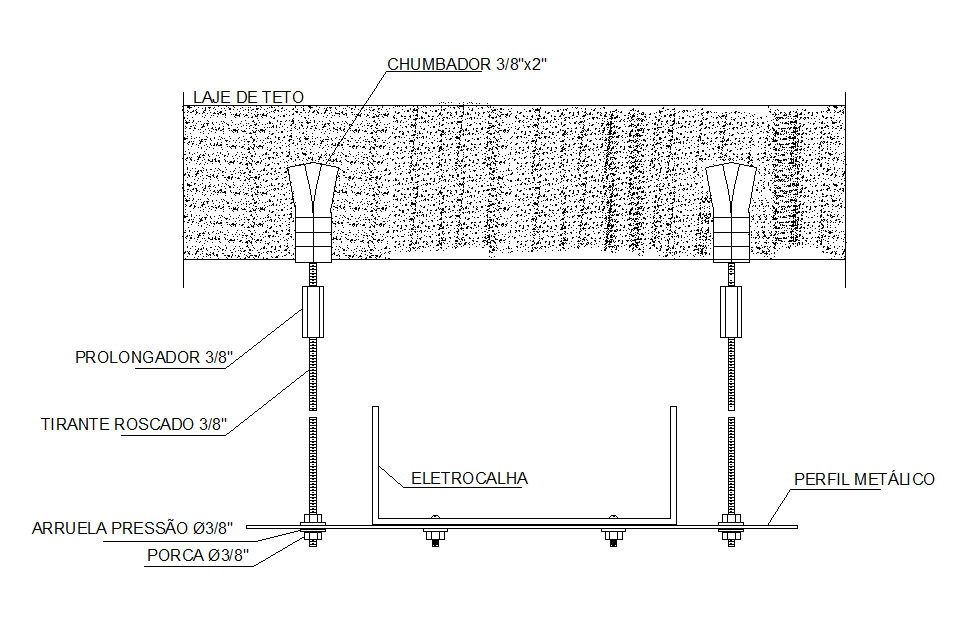
\includegraphics[scale=.30]{Figures/5. Hardware/eletrocalha-fixacao1.png}
		\caption{Eletrocalha fixada através de tirantes}
		\label{fig: eletrocalha fixacao1}
	\end{figure}
	
\end{enumerate}